\section{XUPV5}

En este proyecto se usa la tarjeta Xilinx University Program Virtex 5 (XUPV5).
La tarjeta de desarrollo \emph{XUPV505} es un dispositivo con características
para la evaluación de proyectos de  propósito general, la plataforma de
desarrollo cuenta con memoria incrustrada e interfaces estándar de la industria
de conectividad. Cuenta con el dispositivo FPGA \emph{Virtex-5}.

\subsection{Características de la  tarjeta de desarrollo \emph{XUPV505} }

Las características con las que cuenta la tarjeta de desarrollo son:

\begin{itemize}
 \item FPGA Xilinx \emph{Virtex-5}  
 \item Dos Xilinx XCF32P Flash PROMs (32 Mbyte cada uno) para
configuraciones del dispositivo
 \item Xilinx SystemACE Compact Flash para configuraciones de control
 \item 64-bit 256Mbyte DDR2 small outline DIMM (SODIMM)
 \item 10/100/1000  Interfaces Ethernet 
 \item Intrefaz USB
 \item Sistema de reloj programable
 \item Puerto RS-232
\end{itemize}


\begin{figure}[h!]
 \centering
 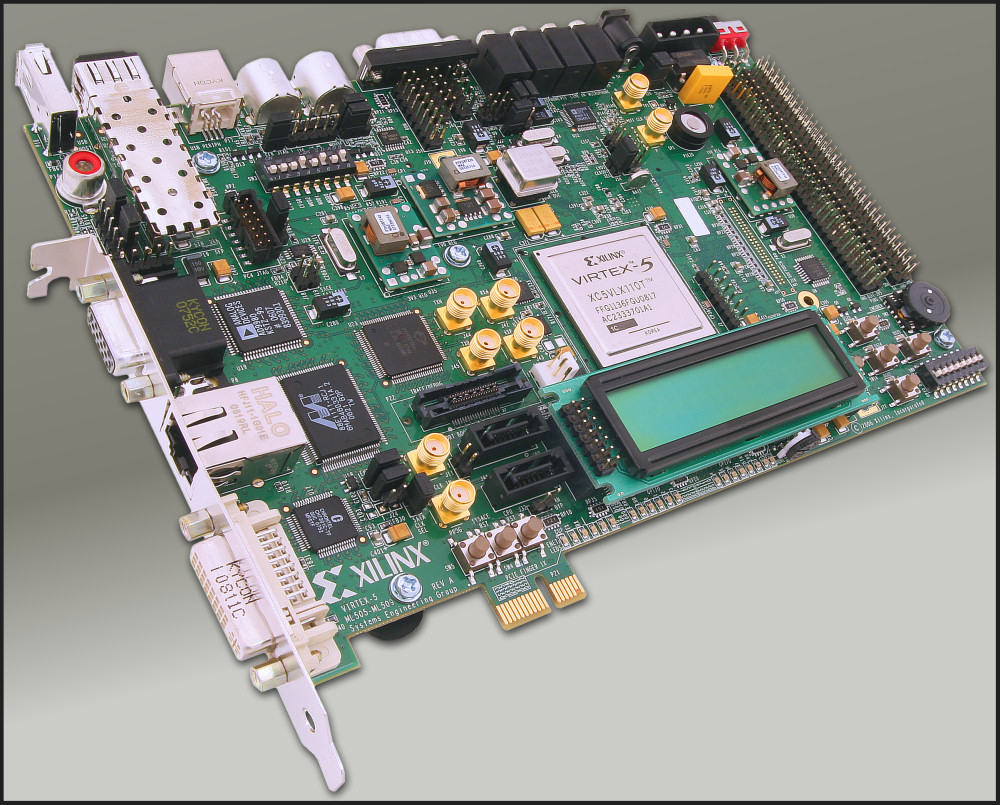
\includegraphics[scale=.30]{./figuras/V5.jpg}
 % V5.jpg: 1000x805 pixel, 72dpi, 35.28x28.40 cm, bb=0 0 1000 805
  \caption{Tarjeta de desarrollo XUPV505}
 \label{XUPV505}
\end{figure}
